%\documentclass[letterpaper, 10pt]{sigcomm-alternate}

\documentclass[peerreview, a4paper, 7pt]{IEEEtran}
%\documentclass[a4paper, 10pt]{IEEEtran}
%\documentclass{scrreprt}
\usepackage{times}
\usepackage{alltt}
\usepackage{graphicx}
\usepackage{alltt}
\usepackage{colortbl}
\usepackage[dvipsnames]{xcolor}
\usepackage{listings}


%\usepackage{color}
% \usepackage{caption2}
%\usepackage{subfigure}
%\usepackage{graphicx}
%\usepackage{colortbl}
%\usepackage[dvipsnames]{xcolor}
% \usepackage{ulem}

\usepackage{hyperref}

\pagenumbering{arabic}


%\ifx\pdfoutput\undefined
%\usepackage[pdfpagemode=none, pdfstartview=FitH, colorlinks=true, urlcolor=black, linkcolor=black, citecolor=black]{hyperref}
%\else
%\usepackage[pdftex, pdfpagemode=none, pdfstartview=FitH, colorlinks=true, urlcolor=black, linkcolor=black, citecolor=black, pdftex]{hyperref}
%\fi

\ifx\HCode\UnDef\else\hypersetup{tex4ht}\fi

%% Editorial work
% \newcommand{\purge}[1]{\textcolor{red}{\sout{#1}}}
% \newcommand{\add}[1]{\textcolor{blue}{#1}}

%%% End of editorial work.


 
\renewcommand{\em}[1]{\textit{#1}}
\begin{document}

\title{Analyzing the IETF ACE-OAuth Protocol}

\author{\authorblockN{Hannes Tschofenig\authorrefmark{1}\\}
\authorblockA{\authorrefmark{3}Arm Limited, 
Email: hannes.tschofenig@arm.com\\}
\thanks{\textsc{Position paper for the '3rd OAuth Security Workshop'~\cite{OSW2018}, x$^{th}$ and x$^{th}$ March 2018, Italy.}}
}

\date{\today}

\maketitle


\section{Abstract}

The OAuth Security Workshop series was started after a group of researchers from Trier/Germany discovery a vulnerability that was found using a formal method analysis of the protocol. Although formal methods have been used in the past for the analysis of Internet security protocols their use still has not become common in the standardization community. If a formal analysis was conducted then this typically happened with the help of researchers rather than by those participating in the standardization process.

In this write-up the author took a recent OAuth specification, namely the ACE-OAuth framework~\cite{draft-ietf-ace-oauth-authz-09}, and uses a formal method to analyze it. The task was simplified using available tools. Initially, Scyther~\cite{Scyther}, developed by Cas Cramer, was used. The Avispa tool was used to verify the results. The use of two tools also offered an impression about the usability. This memo describes the experience using a formal method analysis as well as the result of it. 

In a nutshell, the analyzed specification lacks a description of the security goals. This makes any formal analysis difficult since the person doing the analysis essentially has to make an educated guess of the desired security properties. Furthermore, the Client Token protocol suffers from security flaws. At a minimum, the Client Token protocol either needs to be re-designed or, alternatively, removed from the specification.

\section{ACE-OAuth Overview}
\label{lwm2m}

The high-level architecture of ACE-OAuth is shown in Figure~\ref{ace-oauth-architecture-figure} where the OAuth Client interacts with an Authorization Server to obtain access tokens. Once the OAuth Client is authenticated and authorized (potentially with the consent of the resource owner or some third party) it will receive an access token for use with a Resource Server. The Resource Server hosts the protected resource the OAuth Client is interested to access. Unlike the classical OAuth bearer tokens the access tokens used with ACE-OAuth are a proof-of-possession tokens, which have a key bound to it. When the OAuth Client presents the access token to the Resource Server it also needs to demonstrate possession of the key associated with that access token. 

ACE-OAuth was designed for use in Internet of Things (IoT) environments. As the name indicated it uses the OAuth framework. To make OAuth suitable for use IoT it may be necessary to use CoAP instead of HTTP, DTLS instead of TLS, CBOR instead of JSON, and COSE instead of JOSE. These protocol and encoding alternatives ensure that the payloads transmitted over the air are significantly reduced in size. While such encoding details are not necessarily relevant for a formal analysis they are useful for understanding the goal of the standardization activity in the IETF ACE working group.  

The specification~\cite{draft-ietf-ace-oauth-authz-09} supports a range of different protocol exchanges and analyzing all of them will require a fair amount of time. For this reason the author focused on one exchange, namely the so-called Client Token protocol. This protocol variant was developed with the perceived need to address a very specific deployment limitation: imagine a situation where the OAuth Client is not connected to the Authorization Server to obtain an access token. In this case the OAuth Client needs to relay the communication via the Resource Server to the Authorization Server. This exchange is shown graphically in Figure~\ref{client-token-figure}.

\begin{figure}[!htbp]
 \centering
 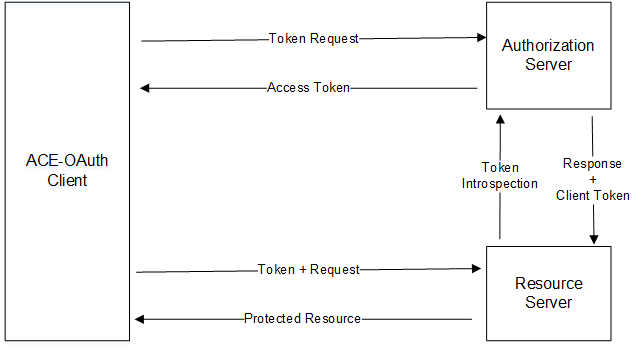
\includegraphics[scale=0.70]{ace-oauth-architecture.png}
 \caption{ACE-OAuth Architecture.}
 \label{ace-oauth-architecture-figure}
\end{figure}

As it can be seen in Figure~\ref{client-token-figure} the protocol starts with the OAuth Client sending a pre-configured access token to the Resource Server, which is then relayed to the Authorization Server via token introspection. The Authorization Server mints keying material (a session key) and conveys it to both the Resource Server and the OAuth Client. The structure used to convey the session key from the Authorization Server to the OAuth Client is via the Client Token (and hence the name Client Token protocol). 

\begin{figure}[!htbp]
	\centering
	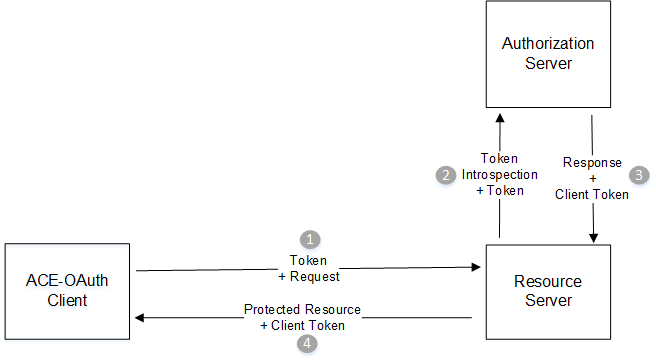
\includegraphics[scale=0.70]{client-token.png}
	\caption{Client Token Protocol.}
	\label{client-token-figure}
\end{figure}

For a formal analysis an appropriate level of abstraction needs to be found. Of course, this process is essential and, if done incorrectly, may prevent to find a vulnerability. Regardless of the formal analysis followed afterwards the step of re-writing the protocol description using a different notation already helps engineers to better understand the completeness of their work. In many cases this step may be more insightful then the actual formal analysis itself. In the example of the Client Token protocol analysis several assumptions had to be made, which are listed below: \\

\begin{description}
	\item[Pre-configured Access Token:] \hfill \\ The specification refers to a pre-configured access token that is stored by the OAuth Client and make the following constraint: "[it] is not self-contained (i.e. it is only a reference to a token at the AS) when it is commissioned". It is essentially an identifier to allow the Authorization Server to select the appropriate key for protection of the Client Token. In the formal analysis the assumption is made that this is just an identifier referring to the OAuth Client. Since an attacker is able to eavesdrops the communication it will be able to learn this pre-configured access token anyway since it is transmitted in cleartext. \\
	\item[Token Introspection:] \hfill \\ The specification does not mandate a specific way to protect the token introspection exchange. We assume that the communication is encrypted. \\
	\item[Proof-of-Possession:] \hfill \\ The specification does not mandate how the OAuth Client demonstrates key confirmation of the established session key with the Resource Server. Since this aspect is not relevant for the illustrated attack we skip it. \\
	\item[Client Token Content:] \hfill \\ The specification only provides basic guidance regarding the content of the Client Token. Those basic recommendations are followed but no additional information is included. \\ 
	\item[Key Distribution:] \hfill \\ The OAuth Client and the Resource Server share a long-term key with the Authorization Server. 
\end{description}


\section{Analysis Result}

Avispa~\cite{Avispa} and Scyther~\cite{Scyther} indicate a vulnerability in the protocol, which is the caused by the lack of authentication of the OAuth Client towards the Authorization Server. This allows an adversary to act as a fake Resource Server. This scenario is not unrealistic given that a token is not required to have any information about the intended recipients nor did the OAuth Client ever express the intended audience in an authenticated way. In a home or industrial environment it is not uncommon that one Resource Server may also act as an OAuth Client in another exchange. Furthermore, one promise of the proof-of-possession token was that it does not require OAuth Client and Resource Server information inside the token but instead only the proof-of-possession key. Figure~\ref{client-token-attack-figure} shows one of the attacks graphically illustrating the lack of the liveness property.

\begin{figure}[!htbp]
 \centering
 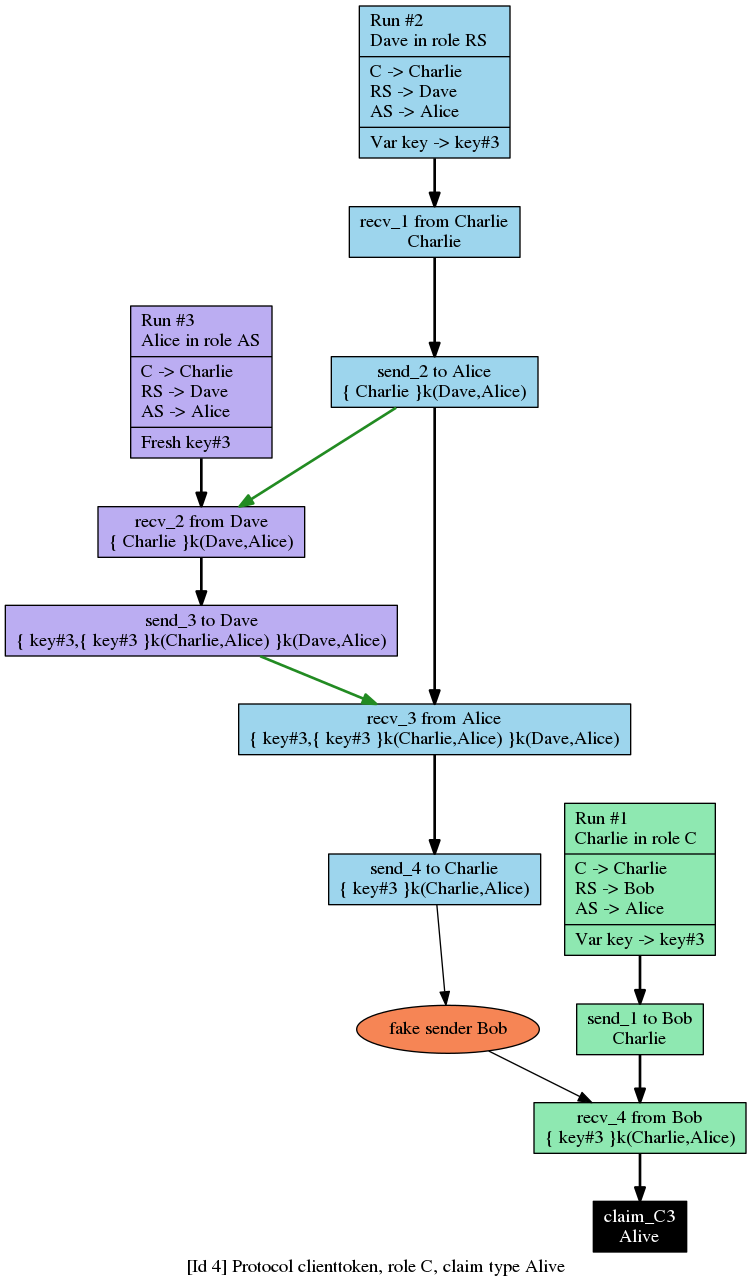
\includegraphics[scale=0.50]{client-token-attack.png}
 \caption{Attack Trace on the Client Token Protocol.}
 \label{client-token-attack-figure}
\end{figure}

The protocol exchange, which is an attack trace produced by the Scyther tool, illustrates three protocol runs (even though two would already be sufficient). In the first protocol run Charlie, acting as an OAuth Client, tries to interact with a Resource Server Bob.  Dave, acting as a rogue Resource server, provides Charlie with the Client Token it had obtained in another protocol run with the Authorization Server Alice. Nothing helps Charlie to notice that it has established communication with Dave instead of with Bob.  

The Client Token protocol can be changed to mitigate this and other attacks. This might, however, lead to the design of a AAA-alike protocol where an authentication protocol has to be defined that runs between the OAuth Client and the Authorization Server. This could be a single, purpose-built pre-shared key protocol or could be designed as a generic authentication framework (like the Extensible Authentication Protocol). Re-using an already specified and analyzed protocol may be the best starting point for such future work. 

\section{Summary and Recommendations}

The OAuth-ACE Client Token protocol was analysed in response to feedback in earlier OAuth security workshops. As researchers had pointed out already in earlier workshops IETF specifications are often too vague to help with the analysis of security properties. While this vague nature may help utilizing the protocol in many different deployment environments and may not even be harmful from an interoperability point of view it leaves a large part of the security analysis to developers, who are most likely not in the best possible position to make such an assessment.

This work therefore aims to create another datapoint in encouraging working groups and specification authors to better articulate the desired security goals of IETF security specifications. Going one step further, the systematic use of formal methods by the working groups will demonstrate maturity in the design process of security protocol. Formal methods allow working group participants to clearly articulate what certain protocol elements offer in terms of security (or what attacks are enabled by their omission). Formal methods, of course, does not replace the need for solid implementations but it will help to improve the overall quality of IETF specifications. 

Ideally, working groups should maintain a repository of already analysed security protocols. This would allow reduce the amount of work by individual authors when defining new extensions to already existing protocols, which is what most IETF working groups do. This would allow to analyse all protocol variants defined in a specification since attention cannot just be focused on the main protocol variant only.

Deciding what formal method technique to use for a given task is complicated since each tool has pros and cons. Scyther, for example, is a recently developed technique with an easy syntax that appears to be easy to use. It does, however, come with limitations in terms of what protocol properties can be analysed. The example code in Appendix~\ref{scyther-code-figure} illustrates how closely the formal description reassembles the protocol description from the specification. The Avispa tool is more powerful but the description is more verbose and more complicated to understand, as one can easily see in Appendix~\ref{avispa-code-figure1,avispa-code-figure2}. Other approaches have been used in the analysis of the OAuth / OpenID protocols, which were considerably more complex. Which approach is best for the analysis of IETF security protocols, where re-use and layering is a common design technique, requires further study. The level of tool support is also a criteria worthwhile to consider in such an evaluation: the Avispa tool, for example, does not appear to be supported to the same extend as more modern techniques like Scyther.

As a concluding thought the author believes that the IETF security community would do itself a favour by studying the use of formal methods to avoid relying extensively on researchers. Creating awareness, for example, at the security area directorate meetings would appear useful. 

\section{Acknowledgments}
I would like to thank TBD for her technical review of this paper. 
 
\bibliographystyle{IEEEtran}
% \bibliographystyle{acmtrans}
\bibliography{paper}

\appendix
\section{Appendix}

\begin{figure}[!htbp]
\begin{lstlisting}
usertype SessionKey;

protocol clienttoken (C,RS,AS)
{
    role C     % C: Client
    {
        var key: SessionKey; 

        send_1(C,RS, C);
        recv_4(RS,C, {key}k(C,AS) );

        claim_C1(C,Secret,key);
        claim_C3(C,Alive);
        claim_C4(C,Weakagree);
        claim_C5(C,Niagree);
        claim_C6(C,Nisynch);
    }        
    role RS     % R: Resource Server
    {
        var key: SessionKey; 

        recv_1(C,RS, C);
        send_2(RS,AS, {C}k(RS,AS)); 
        recv_3(AS,RS,  {key, {key}k(C,AS)}k(RS,AS) ); 
        send_4(RS,C, {key}k(C,AS)); 

        claim_RS1(RS,Secret,key);
        claim_RS3(RS,Alive);
        claim_RS4(RS,Weakagree);
    }    
    role AS     % A: Authorization Server
    {
        fresh key: SessionKey;

        recv_2(RS,AS, {C}k(RS,AS)); 
        send_3(AS,RS, {key, {key}k(C,AS)}k(RS,AS) ); 
    }    
}
\end{lstlisting}
\caption{Client Token Protocol in Scyther Notation.}
\label{scyther-code-figure}
\end{figure}

\begin{figure}[!htbp]
\begin{lstlisting}
% Client Token 

% C: Client
% A: Authorization Server
% R: Resource Server
 
% K_SK: key shared or intended to be shared between C and R
% Initially shared: K_CA, K_RA
	   
% Client
role client_token_C (C, A, R : agent,
                 Snd, Rcv   : channel (dy),
                 K_CA : symmetric_key)
played_by C
def=
  local State           : nat,
        K_SK            : symmetric_key

  const k_cg1, k_cg2 : protocol_id,
        sec_c_K_SK : protocol_id

  init  State := 0

  transition

  1. State = 0 /\ Rcv(start) 
       =|> State':= 1 /\ Snd(C)
  
  2. State = 1 /\ Rcv({K_SK'}_K_CA) 
         =|> State':= 2 
              /\ secret(K_SK',sec_c_K_SK,{C,R,A})		 
		 
end role 


% Resource Server
role client_token_R (R, A, C : agent,
                 Snd, Rcv : channel (dy),
                 K_RA     : symmetric_key)
played_by R
def=
  local State                 : nat,
        K_SK,K_CA             : symmetric_key

  const sec_r_K_SK : protocol_id

  init  State := 0

  transition

  1. State = 0  /\ Rcv(C') =|> 
      State':= 1 /\  Snd({C'}_K_RA)

  2. State = 1 /\ Rcv({K_SK'.{K_SK'}_K_CA}_K_RA) 
         =|> State':= 2 /\ Snd({K_SK'}_K_CA)	  
              /\ secret(K_SK',sec_r_K_SK,{C,R,A})
end role
\end{lstlisting}
\caption{Client Token Protocol in Avispa Notation (Part 1).}
\label{avispa-code-figure1}
\end{figure}

\begin{figure}[!htbp]
\begin{lstlisting}
% Authorization Server
role client_token_A (A, C, R : agent,
                 Snd, Rcv   : channel (dy),
                 K_CA, K_RA : symmetric_key)
played_by A
def=
  local State              : nat,
        K_SK            : symmetric_key

  const k_sk1, k_sk2 : protocol_id,
        sec_a_K_SK : protocol_id

  init  State := 0

  transition

   1. State = 0  /\ Rcv({C}_K_RA) =|> 
      State':= 2 /\ K_SK' := new()
              /\ Snd({K_SK'.{K_SK'}_K_CA}_K_RA) 
              /\ witness(A,C,k_sk1,K_SK')
              /\ witness(A,R,k_sk2,K_SK')
              /\ secret(K_SK',sec_a_K_SK,{A,C,R})
			  	  
end role

role session( C, A, R                             : agent,
              K_CA, K_RA                          : symmetric_key)
def=

   local CR, RC, RA, AR,ARA,RAA : channel (dy)

   composition

   client_token_C (A, C, R, CR, RC, K_CA) 
     /\ client_token_R (R, A, C , RA, AR, K_RA)
	 /\ client_token_A (A, C, R , ARA, RAA, K_CA, K_RA)


end role

role environment() def=

  const  c, a, r, i           : agent,
        kca, kra, kia      : symmetric_key

  intruder_knowledge = {c,a,r,kia}

  composition
        session(c,a,r,kca,kra)
 /\     session(i,a,r,kia,kra)
 /\     session(c,a,i,kca,kia)

end role

goal

  secrecy_of sec_a_K_SK, sec_c_K_SK, sec_r_K_SK
  authentication_on k_sk1 
  authentication_on k_sk2 

end goal
environment()
\end{lstlisting}
\caption{Client Token Protocol in Avispa Notation (Part 2).}
\label{avispa-code-figure2}
\end{figure}

\end{document}

